\documentclass{beamer}

\usepackage[utf8]{inputenc}
\usepackage{default}
\usepackage{amsmath}
\usepackage{tikz}
%\usepackage{chronology}
\usepackage{chronosys}
\usepackage{graphicx}
\usepackage{mwe} % for raisebox
\usepackage{subfig}
\usepackage{multirow}
\usepackage{makecell}%To keep spacing of text in tables
%\renewcommand\cellalign{cc}
\newcommand{\mlcell}[1]{\begin{tabular}{@{}c@{}}#1\end{tabular}}
\usepackage{tabularx} %To do vertical spacing
\usepackage{cellspace}
\setlength\cellspacetoplimit{1pt}
\setlength\cellspacebottomlimit{1pt}
\addparagraphcolumntypes{x, }
\graphicspath{ {./figures/} }

%%%%FROM
%%%%  https://tex.stackexchange.com/questions/312704/chronosys-not-using-only-years
\usepackage{datenumber,xparse}
\usetikzlibrary{arrows.meta,backgrounds}
\newcounter{chronosstartdate}
\newcounter{chronosenddate}
\newcounter{chronosstartyear}
\newcounter{chronosendyear}
\newcounter{chronosyeardate}
\newcounter{chronosthingdate}
\newcounter{chronosotherthingdate}
\pgfkeys{/pgf/number format,
  int detect,
  set thousands separator={},
}
\tikzset{
  chronos/.code={% https://tex.stackexchange.com/a/159856/ - Claudio Fiandrino
    \tikzset{%
      align=center,
      anchor=mid,
      /chronos/.cd,
      #1
    }%
    \setstartyear{\chronosstartyear}%
    \setmydatenumber{chronosstartdate}{\chronosstartyear}{\chronosstartmonth}{\chronosstartday}%
    \setmydatenumber{chronosenddate}{\chronosendyear}{\chronosendmonth}{\chronosendday}%
    \pgfmathsetmacro\chronosunit{(\chronoswidth-20pt)/(\thechronosenddate-\thechronosstartdate)}%
    \draw [line width=\chronosheight] (-10pt,0) coordinate (chronos pre) -- +(\chronoswidth,0) coordinate (chronos post);
    \coordinate (chronos start) at (0,0);
    \coordinate (chronos end) at ([xshift=-10pt]chronos post);
    \setcounter{chronosstartyear}{\chronosstartyear}%
    \setcounter{chronosendyear}{\chronosendyear}%
    \def\tempa{01}%
    \ifx\chronosstartmonth\tempa
      \ifx\chronosstartday\tempa
        \else\stepcounter{chronosstartyear}%
      \fi
      \else\stepcounter{chronosstartyear}%
    \fi
    \def\tempa{12}%
    \def\tempb{31}%
    \ifx\chronosendmonth\tempa
      \ifx\chronosendday\tempb
        \stepcounter{chronosendyear}%
      \fi
    \fi
    \foreach \i in {\thechronosstartyear,...,\thechronosendyear} {%
      \setmydatenumber{chronosyeardate}{\i}{01}{01}%
      \node [above, anchor=south, yshift=.5*\chronosheight] at ({(\thechronosyeardate-\thechronosstartdate)*\chronosunit pt},0) {\i}; }
  },
  chronos set date/.code args={#1-#2-#3:#4}{%
    \tikzset{%
      /chronos/.cd,
      #4 year={#1},
      #4 month={#2},
      #4 day={#3},
    }%
    \setmydatenumber{chronos#4date}{\csname chronos#4year\endcsname}{\csname chronos#4month\endcsname}{\csname chronos#4day\endcsname}%
  },
  chronos date/.style args={#1-#2-#3}{%
    chronos set date/.expanded={#1-#2-#3:thing}%
  },
  chronos period date/.style args={#1-#2-#3}{%
    chronos set date/.expanded={#1-#2-#3:otherthing}%
  },
  /chronos/.search also={/tikz},
  /chronos/.cd,
  start year/.store in=\chronosstartyear,
  start month/.store in=\chronosstartmonth,
  start day/.store in=\chronosstartday,
  end year/.store in=\chronosendyear,
  end month/.store in=\chronosendmonth,
  end day/.store in=\chronosendday,
  thing year/.store in=\chronosthingyear,
  thing month/.store in=\chronosthingmonth,
  thing day/.store in=\chronosthingday,
  otherthing year/.store in=\chronosotherthingyear,
  otherthing month/.store in=\chronosotherthingmonth,
  otherthing day/.store in=\chronosotherthingday,
  start date/.style args={#1-#2-#3}{%
    start year={#1},
    start month={#2},
    start day={#3},
  },
  end date/.style args={#1-#2-#3}{%
    end year={#1},
    end month={#2},
    end day={#3},
  },
  width/.store in=\chronoswidth,
  height/.store in=\chronosheight,
  period/.style={draw=gray},
  period event line/.style={draw=gray, -{Triangle[width=1.5pt, reversed, length=.75pt, fill=gray]}},
  period event/.style={anchor=north, fill=gray!25, draw=gray, rounded corners, align=center, font=\footnotesize},
  event line/.style={draw=gray, -{Triangle[width=1.5pt, reversed, length=.75pt, fill=gray]}},
  event/.style={anchor=north, fill=gray!25, draw=gray, rounded corners, align=center, font=\footnotesize},
  start date=1001-10-01,
  end date=1003-06-14,
  width=100mm,
  height=1pt,
  chronos date=1850-01-01,
  chronos period date=1851-01-01,
}

% It was this
%\NewDocumentCommand \chronosevent { O {} m O {} +m D () { -10pt-.5*\chronosheight } }
% But to overwrite it i had to change it to R (== Required) cfr xparse docs
% and removed the + that is for paragrapht tokens?
\NewDocumentCommand \chronosevent { O {} m O {} m R () { -10pt-.5*\chronosheight } }
{%
  \scoped[on background layer]{\path [postaction={/chronos/event line, #1}, chronos date/.expanded={#2}] ({(\thechronosthingdate-\thechronosstartdate)*\chronosunit pt},0) -- +(0,#5) node [/chronos/event, #3] {\chronosthingday/\chronosthingmonth/\chronosthingyear\\#4};}
}
%Same on this line
\NewDocumentCommand \chronosperiod { O {} m O {} m O {} m R () { -10pt-.5*\chronosheight } }
%\NewDocumentCommand \chronosperiod { O {} m O {} m O {} +m D () { -10pt-.5*\chronosheight } }
{%
  \tikzset{%
    chronos date/.expanded={#2}, chronos period date/.expanded={#4}
  }
  \path [postaction={line width=\chronosheight, /chronos/period, #1}] ({(\thechronosthingdate-\thechronosstartdate)*\chronosunit pt},0) -- ({(\thechronosotherthingdate-\thechronosstartdate)*\chronosunit pt},0);
  \scoped[on background layer]{\path [postaction={/chronos/period event line, #3}] ({(.5*\thechronosotherthingdate+.5*\thechronosthingdate-\thechronosstartdate)*\chronosunit pt},0) -- +(0,#7) node [/chronos/period event, #5] {\chronosthingday/\chronosthingmonth/\chronosthingyear--\chronosotherthingday/\chronosotherthingmonth/\chronosotherthingyear\\#6};}
}
%%%%%% END FROM

\usetheme{CambridgeUS}

\title{Machine Learning @ Becona}
\subtitle{Proof of Concept Image Classification for Concrete Casting Equipment}

\author{Dieter Castel}
\date{\today}

\begin{document}

\begin{frame}
  \titlepage
\end{frame}

\begin{frame}{overview}
\tableofcontents
\end{frame}

\section{Problem}
\begin{frame}{Problem Definition}
  \begin{itemize}
	    \item Automated Sorting of Concrete Casting Equipment 
	    \begin{itemize}
	      \item Exploratory Proof of Concept 
	      \item Focused on Object Recognition Software System
	      \item Educational project for myself 
	    \end{itemize}
	    \item \textbf{Are Convolutional Neural Networks a valid approach for recognizing the Becona rental items?}
  \end{itemize}
\end{frame}

\begin{frame}{Items}
  \begin{itemize}
	    \item About 30 items exist.
	    \item I focused on a subset of 6: \\
	    \begin{tabular}{c|ccc}
	      Id & Name & \# samples & Data Collection Date\\ \hline
	      1 & Spanklem & 223 &  -2017 \\
	      2.0 & Vleugelmoer Opleg Recht - Oud& 208 \\
	      2.1 & Vleugelmoer Opleg Recht - Nieuw& 244 \\
	      3 & Vleugelmoer Opleg Rond & 238 \\
	      4.0 & Variable Spanklem - Kort & 270 \\
	      4.1 & Variable Spanklem - Lang & 251  \\
	    \end{tabular}
	    \item Of which 2.x and 4.x have very high visual similarity
  \end{itemize}
\end{frame}

%TODO: Explain the preiod 1-2
\section{Approach \& Lessons Learned}
\begin{frame}{Hardware \& Software Stack}
\begin{table}
\begin{tabular}{r|cc}
& \textbf{Period 1} & \textbf{Period 2} \\ \hline
Keras &  2.0.6 & \textbf{2.2.2} \\
Tensorflow & 1.3.0 & \textbf{1.13.0} \\
Python & 3.6 & 3.6 \\
cuDNN & 5.1 & \textbf{7.0} \\ 
CUDA & 8.0 & \textbf{9.0} \\
Ubuntu & 16.04.3 LTS & \textbf{fresh 16.04.3 LTS} \\
Storage & Seagate 3TB-7600RPM & \textbf{Samsung 265GB SSD} \\
NVIDIA GPU & \multicolumn{2}{c}{GTX 1060 6GB} \\
Intel CPU &  \multicolumn{2}{c}{Core i5-3570K CPU \@ 3.40GHz} \\
RAM & \multicolumn{2}{c}{16 GB} \\
\end{tabular}
\caption{In P1 trained with testfiles on HDD, later in P2 reinstalled full software stack on new SSD}
\end{table}
\end{frame}

\begin{frame}{5-fold cross-validation}
\begin{figure}
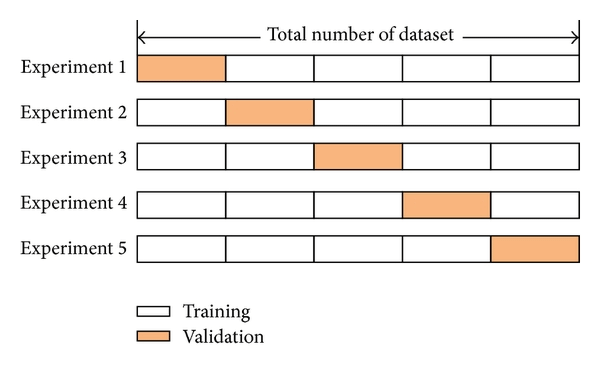
\includegraphics[width=\textwidth]{5foldCV}
%TODO include the figure figures/5-fold-...
%And reference it
\end{figure}
\end{frame}


\begin{frame}
\begin{figure}

\begin{tikzpicture}
  [
    chronos={%
      width=120mm,
      height=10pt,
      start date=2017-08-01,
      end date=2018-12-31,
      period/.style={draw=green},
      event line/.append style={draw=blue},
      period event line/.append style={draw=green},
      event/.append style={fill=blue!25, draw=blue, text=blue},
      period event/.append style={fill=green!25, draw=green!75!black, text=green!75!black},
    }
  ]
  \chronosperiod [draw=red] {2017-09-04} [draw=red] {2017-11-20} [fill=red!25, draw=red, text=red] {First period P1} (40pt+.5*\chronosheight)
  \chronosevent [] {2017-09-04} [] {Acquire first batch of images} (-50pt-.5*\chronosheight)
  \chronosevent [] {2017-09-13} [] {Cropping first batch of Images} (-100pt-.5*\chronosheight)
  \chronosevent [] {2017-08-13} [] {Initial discussion with Jelle} (-10pt -.5*\chronosheight)
  \chronosperiod [] {2018-02-01} [] {2018-07-11} [] {KUL courses} (-20pt-.5*\chronosheight)
\end{tikzpicture}
\end{figure}
\end{frame}

\begin{frame}{LL: Signal/Noise matters}
\begin{itemize}
 \item If signal to noise of image is too large, NN have hard time picking up on the signal.
 \item I learned it the hard way:
\begin{itemize}
 \item First trained with 675 uncropped rectangular images.
 \item Poor training results 
 \item After 1,5h of cropping 675 images.
 \item And retraining the network with squared crops using cropall(ref)
 \item better results ~80\% acc?
\end{itemize}
\end{itemize}
\end{frame}

\begin{frame}{LL: Disk speed matters}
\begin{table}
\caption{Rough estimate: Factor 10 training speed improvement in Period 2}
\begin{tabular}{ccccc}
Period & Experiment ID & CV-split & \mlcell{Approximate \\ Training \\ Hours} & Best Validation Loss \\
1 & mXc\_v5 & split0 & $7$ & $0.17$ \\
1 & mXc\_v6 & split0 & $7$ & $0.2$ \\
1 & mXc\_v5 & split2 & $7$ & $0.16$ \\
1 & mXc\_v6 & split2 & $7$ & $0.18$ \\
2 & mXc\_v5 & split0 & $0.6666$ & $0.25$ \\
2 & mXc\_v6 & split0 & $0.6500$ & $0.22$ \\
2 & mXc\_v5 & split2 & $0.5833$ & $0.2$ \\
2 & mXc\_v6 & split2 & $0.6666$ & $0.22$ \\
\end{tabular}
\end{table}
\end{frame}

\begin{frame}{LL: Latest GPU/Deep Learning libraries matter}
\begin{itemize}
  \begin{itemize}
  \item Upgraded from NVIDIA CUDA 8.0 to CUDA 9.0
  \end{itemize}
\end{itemize}
\end{frame}

\begin{frame}
\begin{itemize}
 \item Training a Neural Network from scratch needs millions of samples 
 \item In two afternoons I took merely 1434 pictures
 \item \textbf{solution}: stand on the shoulder of giants $\rightarrow$ \textbf{transfer learning}
\end{itemize}
\end{frame}

\begin{frame}{Neural Network structure (simplified)}
\begin{figure}
\def\layersep{2.5cm}

\begin{tikzpicture}[shorten >=1pt,->,draw=black!50, node distance=\layersep]
    \tikzstyle{every pin edge}=[-,shorten <=1pt]
    \tikzstyle{neuron}=[circle,fill=black!25,minimum size=17pt,inner sep=0pt]
    \tikzstyle{input neuron}=[neuron];
    \tikzstyle{output neuron}=[neuron];
    \tikzstyle{hidden neuron}=[neuron];
    \tikzstyle{annot} = [text width=4em, text centered]

    % Draw the input layer nodes
    \foreach \id / \x / \y / \rgb / \color in {1/0/0/R/red!50,2/0/0/G/green!30,3/0/0/B/blue!80,4/1/0/R/red}
	\node[input neuron, fill=\color, pin=left:{\rgb-Pixel (\x,\y)}] (I-\id) at (0,-\id) {};

    % Draw the hidden layer nodes
    \foreach \name / \y in {1,...,5}
        \path[yshift=0.5cm]
            node[hidden neuron] (H-\name) at (\layersep,-\y cm) {};

    \foreach \y / \name in {1/1,2/2.0,3/2.1,4/3,5/4.0,6/4.1}
        \path[yshift=0.5cm]
            node[output neuron, pin=right:{$P(\name)$}] (O-\y) at (2*\layersep,-\y cm) {};

    % Connect every node in the input layer with every node in the
    % hidden layer.
    \foreach \source in {1,...,4}
        \foreach \dest in {1,...,5}
            \path (I-\source) edge (H-\dest);

    % Connect every node in the hidden layer with every node in the
    % output layer.
    \foreach \source in {1,...,5}
        \foreach \dest in {1,...,6}
            \path (H-\source) edge (O-\dest);

    % Annotate the layers
    \node[annot,above of=H-1, node distance=1cm] (hl) {Hidden layer\textbf{s}};
    \node[annot,left of=hl] {Input layer}; % 299x299 RGB image
    \node[annot,right of=hl] {Output layer};
    \node[annot,below of=I-2] {$\vdots$};
    \node[annot,below left of=I-3] {$\vdots$};
\end{tikzpicture} 
\end{figure}
\end{frame}

\begin{frame}{Data augmentation 1, 2.0, 2.1}
\begin{figure}
%remove subfigure captions and additional whitespace
\captionsetup[subfigure]{labelformat=empty,farskip=0pt,nearskip=0pt,captionskip=0pt}
\begin{tabular}{cc}
\mlcell{Item \\1.0} &
\raisebox{-0.5\height}{ %centers the image on the line
\subfloat[]{\includegraphics[width = 0.18\textwidth]{aug1-0_1.png}} 
\subfloat[]{\includegraphics[width = 0.18\textwidth]{aug1-0_2.png}} 
\subfloat[]{\includegraphics[width = 0.18\textwidth]{aug1-0_3.png}}
} \\[-2ex] %removes unnecessary vertical whitespace
\mlcell{Item \\ 2.0} &
\raisebox{-0.5\height}{
\subfloat[]{\includegraphics[width = 0.18\textwidth]{aug2-0_1.png}} 
\subfloat[]{\includegraphics[width = 0.18\textwidth]{aug2-0_2.png}} 
\subfloat[]{\includegraphics[width = 0.18\textwidth]{aug2-0_3.png}}
} \\[-2ex] %removes unnecessary vertical whitespace
\mlcell{Item \\ 2.1} &
\raisebox{-0.5\height}{
\subfloat[]{\includegraphics[width = 0.18\textwidth]{aug2-1_1.png}} 
\subfloat[]{\includegraphics[width = 0.18\textwidth]{aug2-1_2.png}} 
\subfloat[]{\includegraphics[width = 0.18\textwidth]{aug2-1_3.png}}
} \\
\end{tabular}
\end{figure}
\end{frame}

\begin{frame}{Data augmentation 3, 4.0, 4.1}
\begin{figure}
%remove subfigure captions and additional whitespace
\captionsetup[subfigure]{labelformat=empty,farskip=0pt,nearskip=0pt}
\begin{tabular}{cc}
\mlcell{Item \\1.0} &
\raisebox{-0.5\height}{ %centers the image on the line
\subfloat[]{\includegraphics[width = 0.18\textwidth]{aug3-0_1.png}} 
\subfloat[]{\includegraphics[width = 0.18\textwidth]{aug3-0_2.png}} 
\subfloat[]{\includegraphics[width = 0.18\textwidth]{aug3-0_3.png}}
} \\[-2ex] %removes unnecessary vertical whitespace
\mlcell{Item \\ 2.0} &
\raisebox{-0.5\height}{
\subfloat[]{\includegraphics[width = 0.18\textwidth]{aug4-0_1.png}} 
\subfloat[]{\includegraphics[width = 0.18\textwidth]{aug4-0_2.png}} 
\subfloat[]{\includegraphics[width = 0.18\textwidth]{aug4-0_3.png}}
} \\[-2ex] %removes unnecessary vertical whitespace
\mlcell{Item \\ 2.1} &
\raisebox{-0.5\height}{
\subfloat[]{\includegraphics[width = 0.18\textwidth]{aug4-1_1.png}} 
\subfloat[]{\includegraphics[width = 0.18\textwidth]{aug4-1_2.png}} 
\subfloat[]{\includegraphics[width = 0.18\textwidth]{aug4-1_3.png}}
} \\
\end{tabular}
\end{figure}
\end{frame}

\section{Results}
\section{Future Work}
\begin{frame}{Advice}
\begin{itemize}
  \item Create Image Capture Pipeline
  \item Multiple-camera's -> vote per camera's == ensemble model
  \item Deploy current best model and monitor wether performance degrades
  \item As soon as enough new samples 
\end{itemize}
\end{frame}{}
\begin{frame}{Technical}
\begin{itemize}
 \item Multi-cameras will give more reliable detection.
 \item Depth sensor (e.g. Microsoft Kinect sensor) will improve accuracy 
  \begin{itemize}
  \item Transfer learning not possible
  \item 
  \end{itemize}
 \item Exploring 3D renderings of the CAD files could help recognition.
\end{itemize}
\end{frame}

\begin{frame}{Project}
\begin{itemize}
 \item Consider collaboration with University.
 \item Master Artificial Inteligence is booming
  \begin{itemize}
  \item Internship students could help create the machine learning pipeline.
  \item Partnership with industry is highly encouraged
  \item  
  \end{itemize}
 \item Depth sensor (e.g. Microsoft Kinect sensor) will improve accuracy 
  \begin{itemize}
  \item Transfer learning not possible
  \item 
  \end{itemize}
 \item Exploring 3D renderings of the CAD files could help recognition.
\end{itemize}
\end{frame}

\section{Q\&A}
\begin{frame}
  \begin{itemize}
	    \item How does the system compare to human classification?
	    \item Speed (vs 24/7), cost (long-term cost hard to estimate), effort, \emph{accuracy}, FP vs FN
	    \item TEST
  \end{itemize}
\end{frame}


\end{document}
